\section{Motor model}
\label{Sect:1}
This section includes the motor rated parameters, key equations, and the analysis of direct and inverse flux maps, as well as the Maximum Torque per Ampere (MTPA) profile.

\subsection{Motor data}
This section presents the key motor parameters extracted from the provided \texttt{Data06.mat} file.

\begin{table}[!h]
    \centering
        \begin{tabular}{@{}lccc@{}} 
        \toprule
        \toprule
        \textbf{Data} & \textbf{Symbol} & \textbf{Quantity} & \textbf{Unit}\\ 
        \midrule
        Stator Resistance      & $R_s$     & 0.127   & $\Omega$ \\
        Apparent Inductance $d$-axis & $L_d$ & ---   & H \\
        Differential Inductance $d$-axis & $LL_d$ & ---   & mH \\
        Apparent Inductance $q$-axis & $L_q$ & ---   & mH \\
        Differential Inductance $q$-axis & $LL_q$ & ---   & mH \\
        Maximum speed          & $n_{\text{max}}$ &---   & rpm \\
        Base speed             & $n_{\text{base}}$ & 3406    & rpm \\
        Maximum torque         & $T_{\max}$ & 71     & Nm \\
        Pole pairs             & $p$       & 3       & -- \\
        \bottomrule
        \end{tabular}
    \captionsetup{justification=justified}
    \caption{Motor data from \texttt{Data06.mat}.}
    \label{tab:Motor_data}
\end{table}

\subsection{Motor equations}
This subsection outlines the voltage and flux equations for a synchronous reluctance machine (SyR), which does not include permanent magnets.

The voltage equation in the $dq$ reference frame is:
\begin{equation}
\mathbf{v}_{dq} = R_s \mathbf{i}_{dq} + \frac{d \boldsymbol{\lambda}_{dq}}{dt} + j \omega \boldsymbol{\lambda}_{dq}
\end{equation}

The flux linkage relationship is:
\begin{equation}
\begin{bmatrix}
\lambda_d \\ \lambda_q
\end{bmatrix}
=
\begin{bmatrix}
L_d(i_d) & 0 \\
0 & L_q(i_q)
\end{bmatrix}
\cdot
\begin{bmatrix}
i_d \\ i_q
\end{bmatrix}
\end{equation}

Since the machine is purely reluctance-based, there is no permanent magnet contribution:
\begin{equation}
\lambda_M = 0
\end{equation}

\subsection{Flux maps and MTPA}
This subsection discusses the direct and inverse flux maps extracted from \texttt{Data06.mat}, as well as the Maximum Torque per Ampere (MTPA) trajectory.

The flux maps are given as:
\begin{itemize}
    \item $\lambda_d = f(i_d, i_q)$ — stored in matrix \texttt{Fd}
    \item $\lambda_q = f(i_d, i_q)$ — stored in matrix \texttt{Fq}
\end{itemize}

\paragraph{Observed characteristics:}
\begin{itemize}
    \item $\lambda_d$ exhibits saturation at high $i_d$
    \item $\lambda_q$ remains approximately linear across most $i_q$ range
\end{itemize}

This confirms that the machine is highly anisotropic, consistent with SyR motor behavior.

\paragraph{Inductance estimation:}

From the flux maps, the differential inductance is calculated as:
\begin{equation}
L_d = \frac{\partial \lambda_d}{\partial i_d}, \quad
L_q = \frac{\partial \lambda_q}{\partial i_q}
\end{equation}

Nominal values used for control design:
\begin{equation}
L_d \approx 0.35 \, \text{mH}, \quad L_q \approx 1.60 \, \text{mH}
\end{equation}

\paragraph{Flux maps:}

\begin{figure}[!ht]
    \centering
    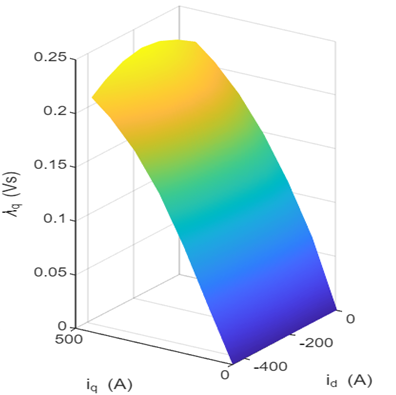
\includegraphics[width=0.8\linewidth]{Figures/Flux map on d axis.png}
    \caption{Flux linkage map on $d$-axis: $\lambda_d$ vs $i_d$ and $i_q$.}
    \label{fig:flux_d}
\end{figure}

\begin{figure}[!ht]
    \centering
    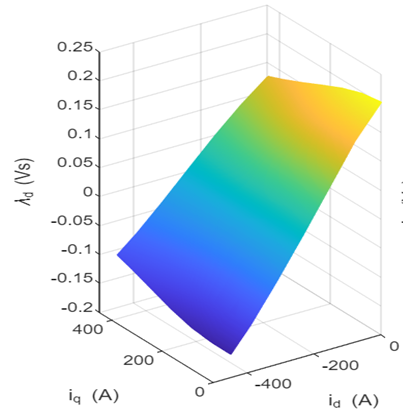
\includegraphics[width=0.8\linewidth]{Figures/Flux map on q axis.png}
    \caption{Flux linkage map on $q$-axis: $\lambda_q$ vs $i_d$ and $i_q$.}
    \label{fig:flux_q}
\end{figure}

\paragraph{MTPA profile:}

The MTPA (Maximum Torque per Ampere) trajectory is available from the vectors:
\begin{itemize}
    \item \texttt{id\_KtMax}, \texttt{iq\_KtMax}, and \texttt{T\_KtMax}
\end{itemize}

This profile defines the optimal $i_d$-$i_q$ current vector that maximizes torque below base speed. It is used in controller reference generation.

% Optional MTPA plot (insert if available)
% \begin{figure}[!ht]
%     \centering
%     \includegraphics[width=0.75\linewidth]{Figures/MTPA_map.png}
%     \caption{MTPA trajectory overlaid with torque contours.}
%     \label{fig:MTPA}
% \end{figure}
